% Chapter 5
\label{Capítulo5}
\chapter{Resultados}
\begin{center}
    \textit{``Newton's third law. You've got to leave something behind''}
     
     Cooper
\end{center}
Os testes foram realizados com o objetivo de validar a implementação do \acrshort{lare} e verificar se os resultados obtidos correspondem aos esperados. A confrontação dos resultados experimentais foi efetuada com recurso ao \href{https://www.multisim.com}{\textit{MultisimLive}}, ao \textit{VirtualBench} e aos valores teóricos previamente descritos na Secção \ref{sec:experiencias}. Para a análise dos resultados, serão apresentados um ou dois exemplos representativos por tipo de experiência, sendo que os restantes são obtidos de forma análoga.

No caso específico da Lei de \textit{Ohm}\footnote{Uma vez que a versão grátis \textit{online} do \textit{MultisimLive} não permite realizar a análise continua - \textit{dc sweep} - esta análise fez-se utilizando o \href{https://www.circuitlab.com/}{CircuitLab}}, há ainda a possibilidade de verificar os valores com recurso a um multímetro de bancada.

As experiências podem ser realizadas com diferentes combinações e configurações:
\begin{itemize}
	\item \textbf{Lei de \textit{Ohm}}: três opções de estudo de resistências;
	\item \textbf{Rectificadores}: quatro combinações possíveis de resistências e condensadores para cada rectificador;
	\item \textbf{Filtros}: duas combinações possiveis de resistências e condensadores para cada filtro.
\end{itemize}

\section{Lei de \textit{Ohm}}
\label{sec:resultados_lei_de_ohm}
O objetivo desta experiência é determinar o valor de uma determinada resistência através do cálculo do declive da recta obtida no gráfico da tensão em função da corrente e, assim, confirmar a Lei de \textit{Ohm}. A Figura \ref{fig:graphohmrepetido}, que novamente aqui se apresenta, representa o gráfico esperado. \textbf{NOTA: Vale a pena? é correcto? Opinião PROF}

\begin{figure}[hbtp]
	\centering
	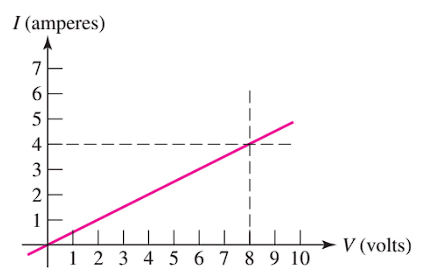
\includegraphics[width=0.3\textwidth]{figures/grafico_Ohm.png}
	\caption{Gráfico da Lei de \textit{Ohm}}
	\label{fig:graphohmrepetido}
\end{figure}

\subsection{Resultados prácticos}
\label{sec:resultados_praticos}
Como já foi referido - VER REFERÊNCIA - o utilizador efectua cinco medições de cada grandeza (tensão e corrente), para uma das três resistências disponíveis.

Na Figura \ref{fig:resultados_medicoes_1k} está representado o resultado de um par de medições para uma resistência de \SI{1}{\kilo\ohm}. As restantes medições, em intervalos de \SI{1}{\volt} até \SI{5}{\volt}, são obtidas de forma análoga.

\begin{figure}[hbtp]
	\centering
	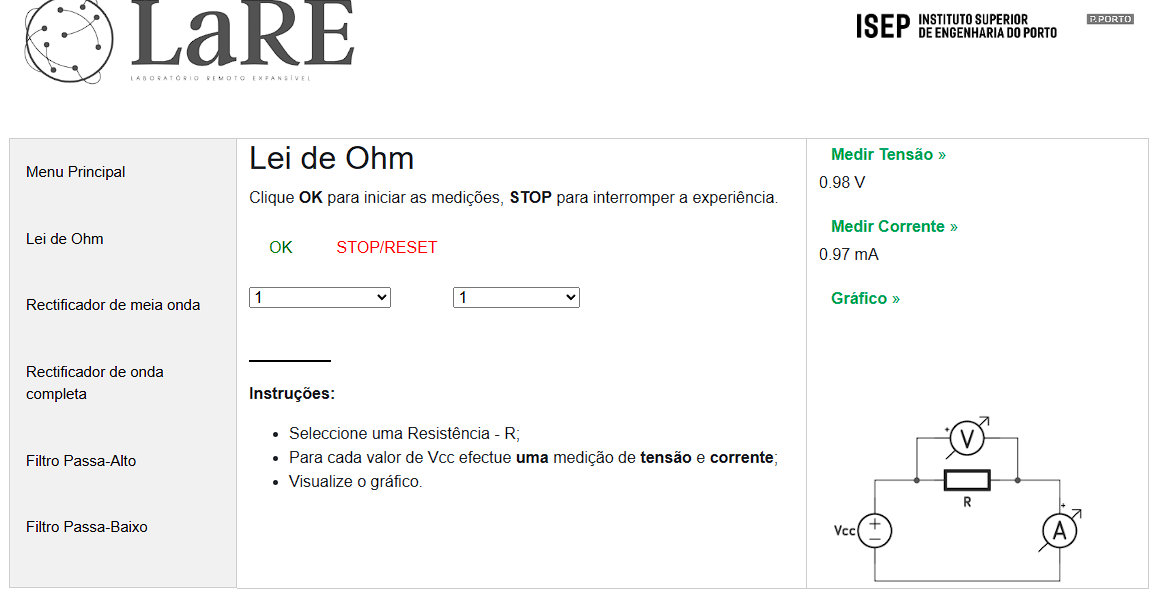
\includegraphics[width=0.7\textwidth]{figures/resultados_medicoes_ohm.png}
	\caption{Medição práctica}
	\label{fig:resultados_medicoes_1k}
\end{figure}

O valor real da resistência, obtida por medição directa, é de \SI{998}{\ohm}, estando dentro da tolerância que é de $\pm$5\%.

O erro associado aos instrumentos de medição pode ser considerado desprezável. De acordo com as especificações do modelo \textit{VB-8012}\cite{datasheetvb8012}, a precisão para medições de tensão em corrente contínua é:

\begin{itemize}
	\item Faixa de \SI{1}{\volt}
	\begin{itemize}
		\item Precisão garantida (1 ano): $\pm$(0.015\% da leitura $\pm$ 0.005\% da faixa)
	\end{itemize}
\end{itemize}

Estes valores indicam que, para uma leitura de \SI{1}{\volt}, o erro máximo estimado devido à precisão do instrumento seria de, aproximadamente $\pm$\SI{0.0002}{\volt}, ou seja, $\pm$\SI{0.2}{\milli\volt}.

Portanto, a diferença entre a tensão fornecida pela fonte — \SI{1}{\volt} — e os valores medidos — \SI{0.98}{\volt} e \SI{0.97}{\milli\ampere} — deve-se, principalmente, à tolerância da resistência utilizada. Assim, conclui-se que os valores medidos se encontram dentro dos limites expectáveis, sendo perfeitamente aceitáveis face às tolerâncias envolvidas.

O gráfico \textit{U vs I}, obtido para esta resistência é apresentado na Figura \ref{fig:grafico_LaRE_1k}. O declive da recta, que representa a resistência, foi calculado e confrontado com o valor real da resistência. 

\begin{figure}[hbtp]
	\centering
	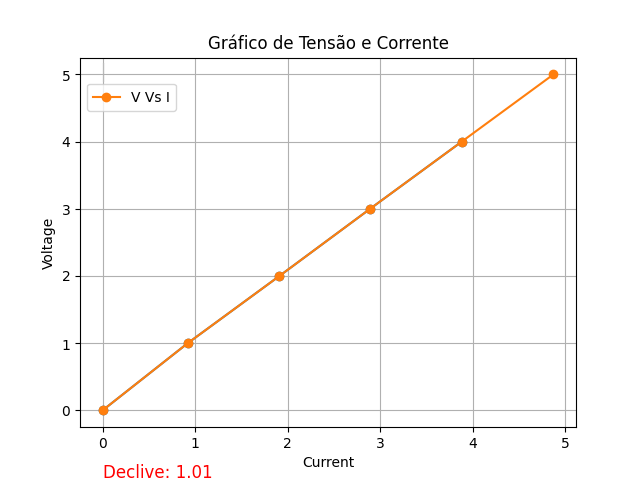
\includegraphics[width=0.7\textwidth]{figures/ohm_graph.png}
	\caption{Gráfico da Lei de \textit{Ohm} - \SI{1}{\kilo\ohm} - MUDAR}
	\label{fig:grafico_LaRE_1k}
\end{figure}

O erro relativo entre o valor teórico(real) e o valor obtido experimentalmente, pode ser calculado através da Equação \ref{eq:errorelativo}:

\begin{equation} \label{eq:errorelativo}
	\text{Erro Relativo} = \frac{|R_{real} - R_{obtido}|}{R_{real}} \times 100
\end{equation}

No caso descrito em cima, o erro relativo obtido é de, aproximadamente, \SI{1.2}{\percent}, sendo um valor perfeitamente aceitável.

Ainda assim e como forma de complementar a análise dos resultados, foram efectuados testes complementares usando dois simuladores, neste caso, o \href{https://www.multisim.com}{\textit{MultisimLive}} e o \href{https://www.circuitlab.com/}{\textit{CircuitLab}}. A Figura \ref{fig:multisimOHM} e a Figura \ref{fig:circuitlab} mostram os resultados obtidos.

\begin{figure}[hbtp]
	\centering%
		\centering
		\subfloat[\centering Multisim\label{fig:multisimOHM}]{{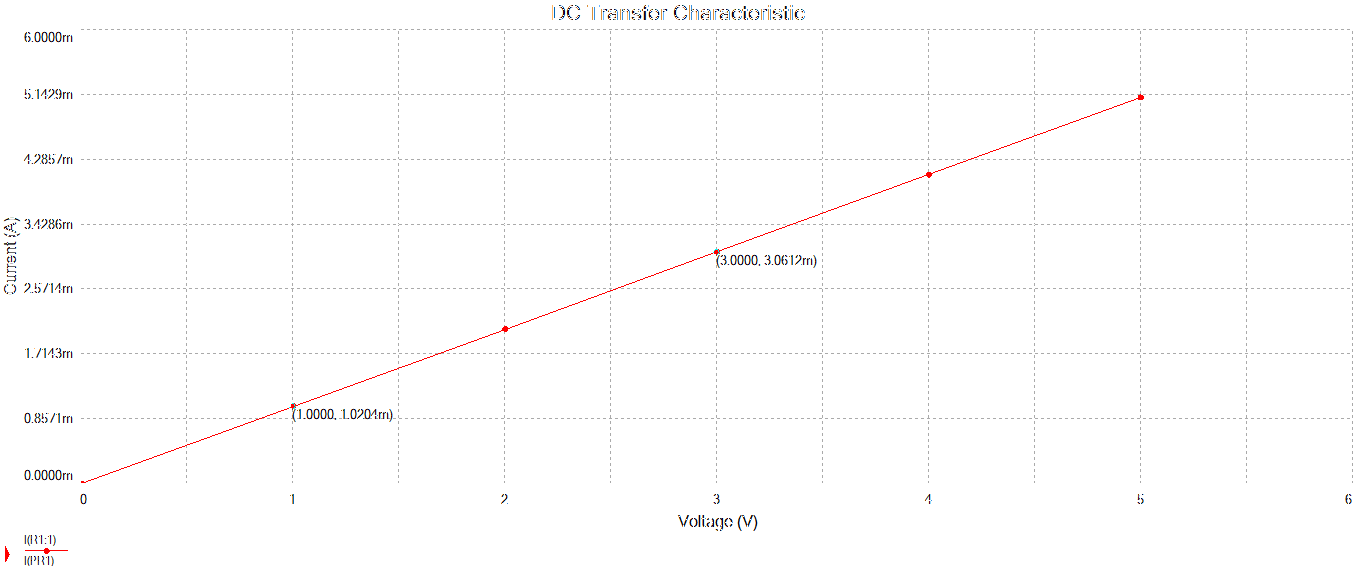
\includegraphics[width=6.3cm]{figures/OHM_resultado_multisim.png} }}%
		\qquad
		\subfloat[\centering CircuitLab\label{fig:circuitlab}]{{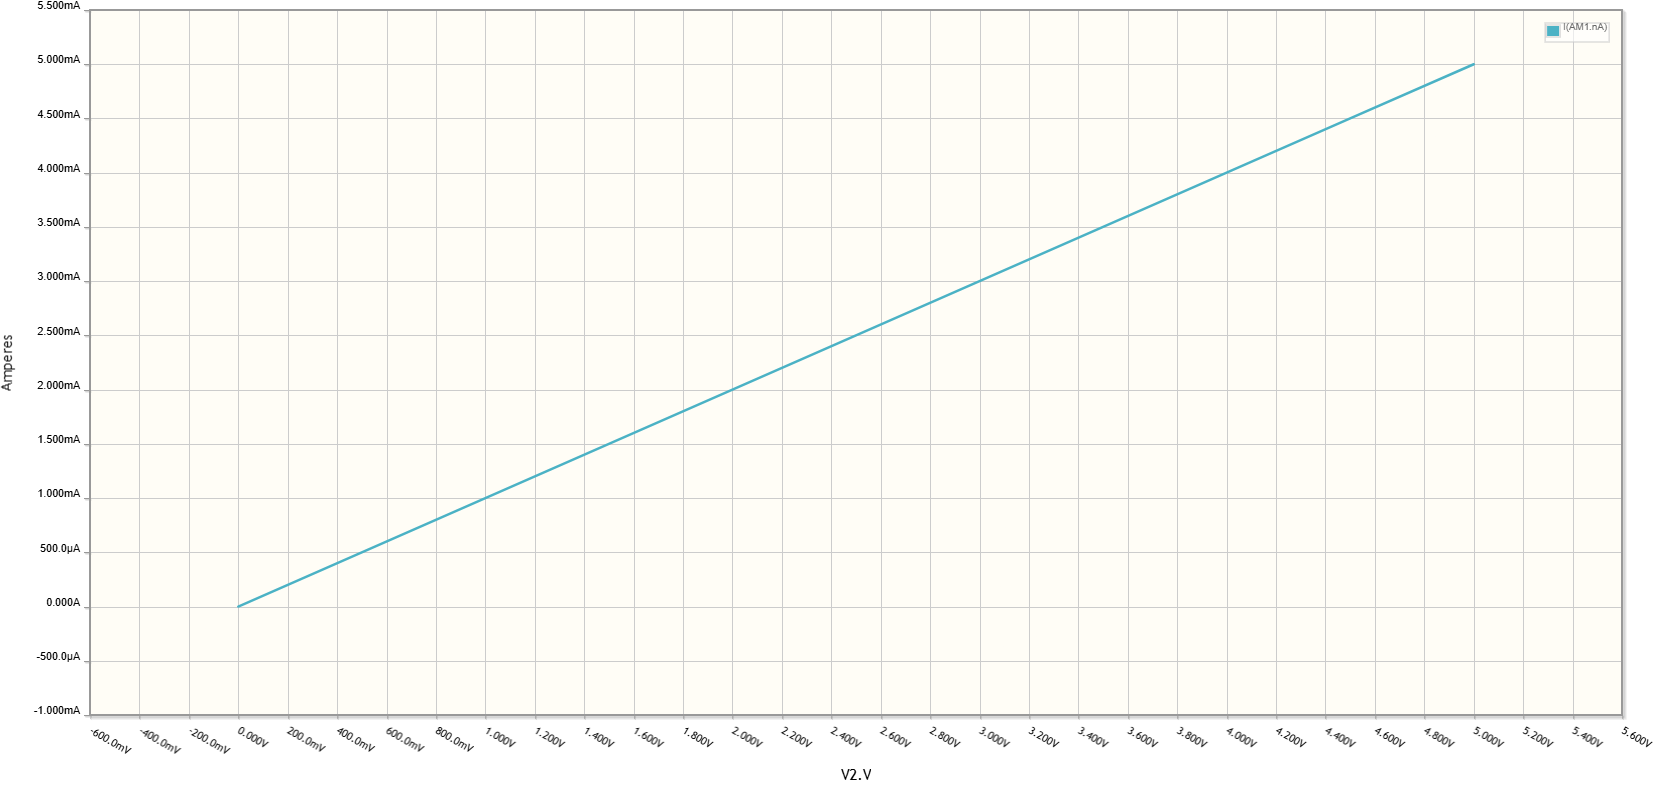
\includegraphics[width=6.3cm]{figures/OHM_resultado_circuitlab.png} }}%
		\caption{Experiência Lei de \textit{Ohm}}%
		\label{fig:experienciaOHM_simuladores}%
	\end{figure}

Através da análise do gráfico obtido no \textit{MultisimLive} e no \textit{CircuitLab} é possível calcular os declives das rectas, dados pela Equação \ref{eq:declive}

\begin{equation} \label{eq:declive}
	\text{m} = \frac{y_{b} - y_{a}}{x_{b} - x_{a}}
\end{equation}

O valor do declive, correspondente à resistência, obtido para estes dois simuladores é, respectivamente, $m_\text{{multisim}} \approx{0.980}$ e $m_{\text{CircuitLab}} \approx{1.002}$. Tendo em conta que a escala do eixo do $y$ está representada em \SI{}{\milli\ampere}, os valores das resistências surgem expressos em \SI{}{\kilo\ohm}, isto é, $R_\text{{multisim}} = \SI{0.980}{\kilo\ohm}$ e $R_{\text{CircuitLab}} = \SI{1.002}{\kilo\ohm}$.  Assim aplicando a Equação~\ref{eq:errorelativo} obtém-se um erro relativo de \SI{1.80}{\percent} e \SI{0.4}{\percent}, respectivamente.

Pela análise dos gráficos obtidos, conclui-se que os resultados obtidos com o \acrshort{lare} são semelhantes aos obtidos com os simuladores e aos valores reais.

\section{Rectificadores}
As duas experiências foram implementados com o objectivo de estudar e avaliar a tensão de \textit{ripple} nos circuitos rectificadores de meia onda e onda completa, considerando as quatro combinações possíveis dos pares resistência/condensador. COLOCAR REFERÊNCIA.

As formas de onda esperadas estão representadas na Figura \ref{fig:sedraripple} e Figura \ref{fig:sedraripplecompleta} sendo os valores teóricos da tensão de \textit{ripple} determinados pela Equação \ref{eq:vripple} e Equação \ref{eq:vrippleOC}. \textbf{NOTA: Aqui coloquei a referência às imagens, ao contrário da Lei de ohm. Opinião PROF}

\subsubsection{Filtros}
\label{sec:filtros}
Representados na Figura \ref{fig:filtrosesqgeral} estão os filtros simplificados, leccionados em contexto de sala de aula no ensino secundário.

A possibilidade de variar a frequência do sinal de entrada permite que estas experiências sejam utilizadas para estudar a resposta em frequência dos filtros, analisar o Diagrama de \textit{Bode}, determinar a frequência de corte dada pela Equação \ref{eq:frequenciacorte} e ainda relacionar, por exemplo, o valor da tensão de entrada com a tensão de saída. 

\begin{equation} \label{eq:frequenciacorte}
	f_{c} = \frac{1}{2\pi RC}
\end{equation}

\begin{comment}
	\textbf{Acho que não é necessário referir a relação entre a tensão de entrada e a tensão de saída, já que isso é feito na parte de software. O que se pode fazer é referir que o \acrshort{lare} permite estudar a resposta em frequência dos filtros, analisar o Diagrama de \textit{Bode} e determinar a frequência de corte.}
A Figura \ref{fig:diagramabode} apresenta um exemplo do Diagrama de \textit{Bode} de um filtro passa-alto, obtido nos testes do LaRE.

\begin{figure}[hbtp]
	\centering
	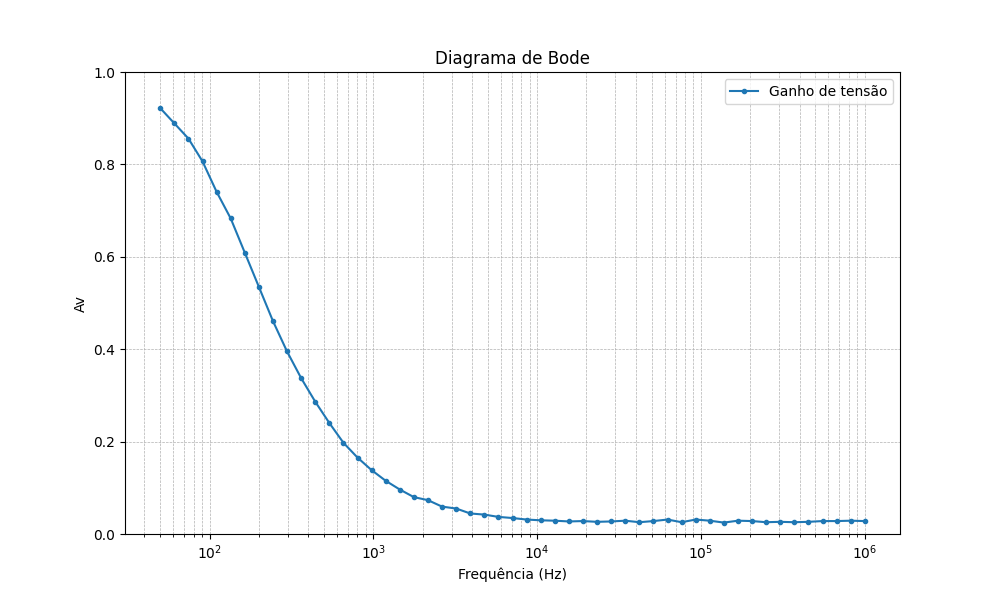
\includegraphics[width=0.6\textwidth]{figures/bode_lpf.png}
	\caption{Diagrama de \textit{Bode} - Filtro passa-alto}
	\label{fig:diagramabode}
\end{figure}
\end{comment}

As Figuras \ref{fig:Bode_pb} e \ref{fig:Bode_pa} apresentam os Diagramas de \textit{Bode} \textins{ideais}, que servem de referência para o estudo desta experiência. 

\begin{figure}[hbtp]
	\centering%
		\centering
		\subfloat[\centering Filtro passa-baixo\label{fig:Bode_pb}]{{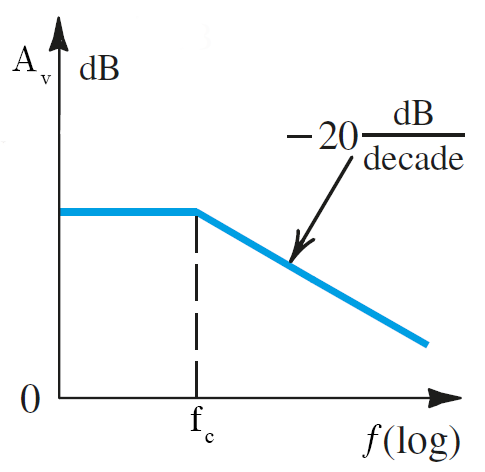
\includegraphics[width=6cm]{figures/Sedra_BodeFPB.png} }}%
		\qquad
		\subfloat[\centering Filtro passa-alto\label{fig:Bode_pa}]{{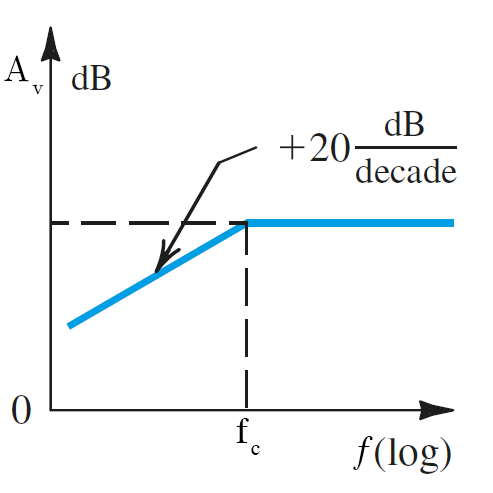
\includegraphics[width=6cm]{figures/Sedra_BodeFPA.png} }}%
		\caption{Diagramas de \textit{Bode} \textins{ideal} \cite{sedrasmith}}%
		\label{fig:Bodeesqgeral}%
\end{figure}

	Para além da análise em frequência, um outro aspeto complementar a considerar é a relação entre as ondas de entrada e saída, em função da frequência. Nos filtros, o intervalo de frequências permitido é igual ao já referido para os rectificadores: entre \SI{50}{\hertz} a \SI{2000}{\hertz}. 
	
	A frequência de corte de um filtro é definida como o ponto onde o ganho do filtro sofre uma atenuação de \SI{3}{\decibel} em relação ao seu valor máximo. 	Para um filtro passa-baixo (passa-alto) ideal, o ganho em baixas (altas) frequências é unitário. Quando o sinal atinge a frequência de corte, a relação entre a tensão de saída e a tensão de entrada reduz-se para:  
	
	\begin{equation} \label{eq:relacaoGanho}
		\frac{U_{out}}{U_{in}} = \frac{1}{\sqrt{2}} \approx 0.707
	\end{equation}
	
	\ldots ou na escala logarítmica:  
\begin{equation} \label{eq:relacaoGanhodB}
	\frac{U_{out}}{U_{in}} = 20 \log_{10} (0.707) \approx -\SI{3}{\decibel}	
\end{equation}
	
Assim, a frequência de corte de um filtro corresponde ao ponto em que a amplitude do sinal de saída é aproximadamente $70.7\%$ da amplitude do sinal de entrada, o que corresponde a -\SI{3}{\decibel}. 


\textbf{Tal como o prof disse, refrerir que os valores, imagem, iformação e enviada para a página via xpto, blá, blá, através do ficheiro, flask, tal como referido no cap tal - referir também como é enviada a string}

\textbf{DE UMA FORMA BREVE E RESEUMIDA, REFERIR QUANTO BITS E COMO SE FAZ A COMUNICAÇÃO COM O SER}

13 bits começar pelo esquema completo antes de dar os exemplos de funcionamento. a explicação penso que pode ficar dividida como está, mas já com o esquema e relés com os indices certos, a explicação mas os exemplos descritos em tabela só fazem sentido se for o esquema completo,


\section{Limitações}
\section{Melhoramentos}


